\documentclass{beamer}

\usetheme{Warsaw}
\usefonttheme[onlylarge]{structurebold}
\useinnertheme{rectangles}
\setbeamerfont*{frametitle}{size=\normalsize,series=\bfseries}
\setbeamertemplate{navigation symbols}{}

\usepackage[polish]{babel}
\usepackage[utf8]{inputenc}
\usepackage{times}
\usepackage[T1]{fontenc}
\usepackage{listings}
\usepackage{graphicx}
\usepackage{enumerate}
\usepackage[normalem]{ulem}
\usepackage{bussproofs}

\definecolor{ugreen}{rgb}{0, 0.5, 0}
\definecolor{lgreen}{rgb}{0.85, 1, 0.85}
\definecolor{annot}{rgb}{0.7, 0, 0}
\definecolor{lstback}{RGB}{235 240 250}

\setbeamercolor{gr}{fg=white, bg=ugreen}
\setbeamercolor{lgr}{fg=black, bg=lgreen}

\setcounter{tocdepth}{1}
\AtBeginSection[]
{
  \begin{frame}<beamer>{Outline}
    \tableofcontents[currentsection, hideothersubsections]
  \end{frame}
}

\title{JSR 308 i weryfikacja adnotacji Javy}

\author{Sławomir Rudnicki} 

\institute{Niezawodność systemów współbieżnych i obiektowych}

\date{27 października 2010}

\lstset{language=Java, showstringspaces=false, backgroundcolor=\color{lstback}, 
        emph={@NonNull, @Nullable, @SuppressWarnings, @Deprecated, @UTF8, 
              @Id, @Length, @UserPrincipal, @Target, @Retention, @interface, 
              @Entity, @GeneratedValue, @Existing, @ReadOnly, 
              @Readonly, @Critical, @TypeQualifier, @SubtypeOf, @ImplicitFor,
              @Immutable, @NonEmpty}, 
        emphstyle={\color{annot}}, 
        columns=fullflexible}

\begin{document}

\begin{frame}
  \titlepage
\end{frame}
\begin{frame}
  \tableofcontents[pausesections]
\end{frame}

\setcounter{tocdepth}{2}

\section{Wprowadzenie}

\begin{frame}{Sfera zainteresowań na dziś}
\begin{itemize}
\item[$\rightarrow$] weryfikacja własności elementów programu:
\begin{itemize}
\item klas, 
\item metod, 
\item obiektów, 
\item pól obiektów...
\end{itemize}
\end{itemize}
\end{frame}

\begin{frame}{Sfera zainteresowań na dziś}
\begin{itemize}
\item<1->[$\rightarrow$] własności definiowane przy pomocy \textbf{adnotacji}
\begin{center}
\lstinputlisting{code/annot-example.java}
\end{center}
\item<2->[$\rightarrow$] weryfikacja będzie odbywać się \textbf{statycznie} -- analiza kodu źródłowego
\end{itemize}
\end{frame}

\section{Adnotacje}
\subsection{Historia}
\begin{frame}{Adnotacje w Java 5}
\begin{itemize}
\item<1-> Adnotacje zostały wprowadzone w Javie 5 na podstawie propozycji
  JSR 175 z 2002 roku.
\item<2-> Cel: 
\begin{itemize}
\item umożliwienie wprowadzania metadanych do kodu źródłowego
\end{itemize}
\item<3-> Postać adnotacji: 
\begin{itemize}
\item \color{red} @NonNull 
\item \color{red} @Deprecated
\item \color{red} @Length(min=6, max=50)
\end{itemize}
\end{itemize}
\end{frame}

\begin{frame}{Adnotowane elementy}
  \structure{Klasy}  
  \lstinputlisting{code/annot-class.java}
  \pause
  \structure{Metody i konstruktory}
  \lstinputlisting{code/annot-method.java}
\end{frame}

\begin{frame}{Adnotowane elementy}
  \structure{Parametry metod}
  \lstinputlisting{code/annot-param.java}
  \pause
  \structure{Pola klas}
  \lstinputlisting{code/annot-field.java}
\end{frame}

\subsection{Własne adnotacje}

\begin{frame}{Własne adnotacje}
\begin{itemize}
\item W Java 5.0 zostały wbudowane tylko trzy adnotacje:
\begin{itemize}
\item \color{red} @Deprecated
\item \color{red} @SuppressWarnings
\item \color{red} @Override
\end{itemize}
\pause
\item Programista może łatwo tworzyć własne adnotacje
\end{itemize}
\end{frame}

\begin{frame}{Przykład definicji adnotacji}
\lstinputlisting{code/custom-annot.java}
\end{frame}

\begin{frame}{@Retention}
Określa zasięg adnotacji:
\begin{description}[RUNTIME]
\item<1->[SOURCE] -- ignorowane przez kompilator
\item<2->[CLASS] -- zachowywane w pliku \texttt{.class}, niewidoczne w czasie
  wykonania
\item<3->[RUNTIME] -- widoczne w czasie wykonania, mogą być interpretowane
  przez JVM.
\end{description}
\end{frame}

\begin{frame}{@Target}
Określa, jakie elementy mogą być adnotowane:
\begin{itemize}[ANNOTATION\_TYPE]
\item<1-> PACKAGE -- deklaracja pakietu
\item<2-> TYPE -- klasy, interfejsy i wyliczenia
\item<3-> CONSTRUCTOR $\quad$
\item<3-> METHOD $\quad$
\item<4-> PARAMETER $\quad$
\item<4-> FIELD $\quad$
\item<4-> LOCAL\_VARIABLE $\quad$
\item<5-> ANNOTATION\_TYPE -- meta-adnotacje
\end{itemize}
\end{frame}

\begin{frame}{Zastosowania}
Adnotacje znalazły szerokie zastosowanie, przyczyniając się 
do rozwoju frameworków platformy J2EE.
\begin{itemize}
\item metadane można definiować bezpośrednio w kodzie, 
  a nie w dodatkowych plikach.
\end{itemize}
\pause
Przewaga nad JML-em: 
\begin{itemize}
\item adnotacje mogą być zachowane w plikach \texttt{.class}
\end{itemize}
\end{frame}

\begin{frame}{Adnotacje w J2EE: Hibernate}
  \textbf{Hibernate Mapping:}
  \lstinputlisting[language=XML]{code/hibernate.xml}
\end{frame}

\begin{frame}{Adnotacje w J2EE: Hibernate}
  \textbf{Hibernate Annotations:}
  \lstinputlisting{code/hibernate.java}
\end{frame}

\section{JSR 308}
\subsection{Wprowadzenie}
\begin{frame}{JSR 308}
Propozycja rozszerzenia składni Javy o możliwość adnotowania
\emph{wszystkich wystąpień} nazwy typu.
\pause
\begin{itemize}
\item projekt -- rok 2006
\item w założeniu -- część standardu Java 7.
\end{itemize}
\end{frame}

\subsection{Rozszerzenia składni}

\begin{frame}{JSR 308: rozszerzenia składni}
  Można adnotować:
  \begin{itemize}
  \item<1-> każde wystąpienie nazwy typu
  \item<2-> obiekt będący odbiorcą metody
  \item<3-> parametry formalne typów generycznych
  \item<4-> maskę \texttt{?} stanowiącą parametr typu generycznego
  \item<5-> poszczególne poziomy zagnieżdżenia typów tablicowych (\texttt{[]})
  \end{itemize}
\end{frame}

\subsection{Przykłady}

\begin{frame}{Przykłady}
  \structure{Argumenty typów generycznych}
  \lstinputlisting{code/jsr-generics.java}
  \structure{Argumenty metod generycznych}
  \lstinputlisting{code/jsr-gen-meth.java}
\end{frame}

\begin{frame}{Przykłady}
  \structure{Ograniczenia argumentów typów generycznych}
  \lstinputlisting{code/jsr-gen-bounds.java}
  \structure{Parametry formalne typów generycznych}
  \lstinputlisting{code/jsr-gen-formal.java}
\end{frame}

\begin{frame}{Przykłady}
  \structure{Opis nadklas i interfejsów}
  \lstinputlisting{code/jsr-superclass.java}
  \structure{Wyjątki}
  \lstinputlisting{code/jsr-exception.java}
\end{frame}

\begin{frame}{Przykłady}
  \structure{Odbiorcy dla metod}
  \lstinputlisting{code/jsr-receiver.java}
  \structure{Wyniki konstruktorów}
  \lstinputlisting{code/jsr-construct.java}
\end{frame}

\begin{frame}{Przykłady}
  \structure{Tablice}
  \lstinputlisting{code/jsr-array.java}
\end{frame}

\begin{frame}{Przykłady}
  \structure{Rzutowanie}
  \lstinputlisting{code/jsr-cast.java}
  \structure{Tworzenie obiektów}
  \lstinputlisting{code/jsr-creation.java}
\end{frame}

\subsection{Co dalej?}

\begin{frame}{Propozycje rozwoju adnotacji}
  \begin{itemize}
  \item<1-> adnotacje dla wyrażeń
% Brak przypadków użycia
  \item<2-> adnotacje dla instrukcji
% Własności wykonania: atomowość/współbieżność. Projekt w toku.
  \item<3-> dziedziczenie adnotacji
% W tej chwili można dziedziczyć adnotacje klas, jeżeli jest ustawiona
% meta-adnotacja @Inherited. Twórcy sądzą, że przydatne może być
% dziedziczenie adnotacji na metodach/polach oraz dziedziczenie z
% implementowanych interfejsów
  \end{itemize}
\end{frame}

\begin{frame}{Krytyka}
  Michael Nygard, \emph{When Should You Jump? JSR 308. That's When.}\only<2->{:}
  \pause
  \begin{quote}
Every language has a complexity budget. Java blew through it with
generics in Java 5. Now, seriously, take another look at this:
  \end{quote}
  \lstinputlisting{code/nygard.java}
  \begin{quote}
    Does that even look like Java? 
  \end{quote}
\end{frame}

\begin{frame}{Dalsze losy}
  \begin{itemize}
  \item<1-> JSR 308 nie wejdzie do standardu Java 7 
    \begin{itemize}
    \item odroczony do wersji 8 lub późniejszej
    \end{itemize}
  \item<2-> Mimo to projekt jest aktywny:
    \begin{itemize}
    \item Powstały narzędzia typu \emph{proof of concept}
    \item Kompilator OpenJDK Javy 7 rozumie rozszerzoną składnię
    \end{itemize}
  \end{itemize}
\end{frame}

\section{Weryfikacja adnotacji}
\subsection{Wprowadzenie}

\begin{frame}{Weryfikacja adnotacji}
\begin{itemize}
\item<1-> Adnotacje mogą opisywać własności programu, które powinny
  zostać przetworzone w czasie kompilacji programu.
\item<2-> W tym celu możliwe jest definiowanie \emph{procesorów
  adnotacji} (annotation processors) i włączanie ich w tok
  kompilacji programu.
  \begin{itemize}
  \item W standardowej Javie do tego celu służy narzędzie \texttt{apt}
  \end{itemize}
\end{itemize}
\end{frame}

\subsection{apt}

\begin{frame}{Schemat działania}
  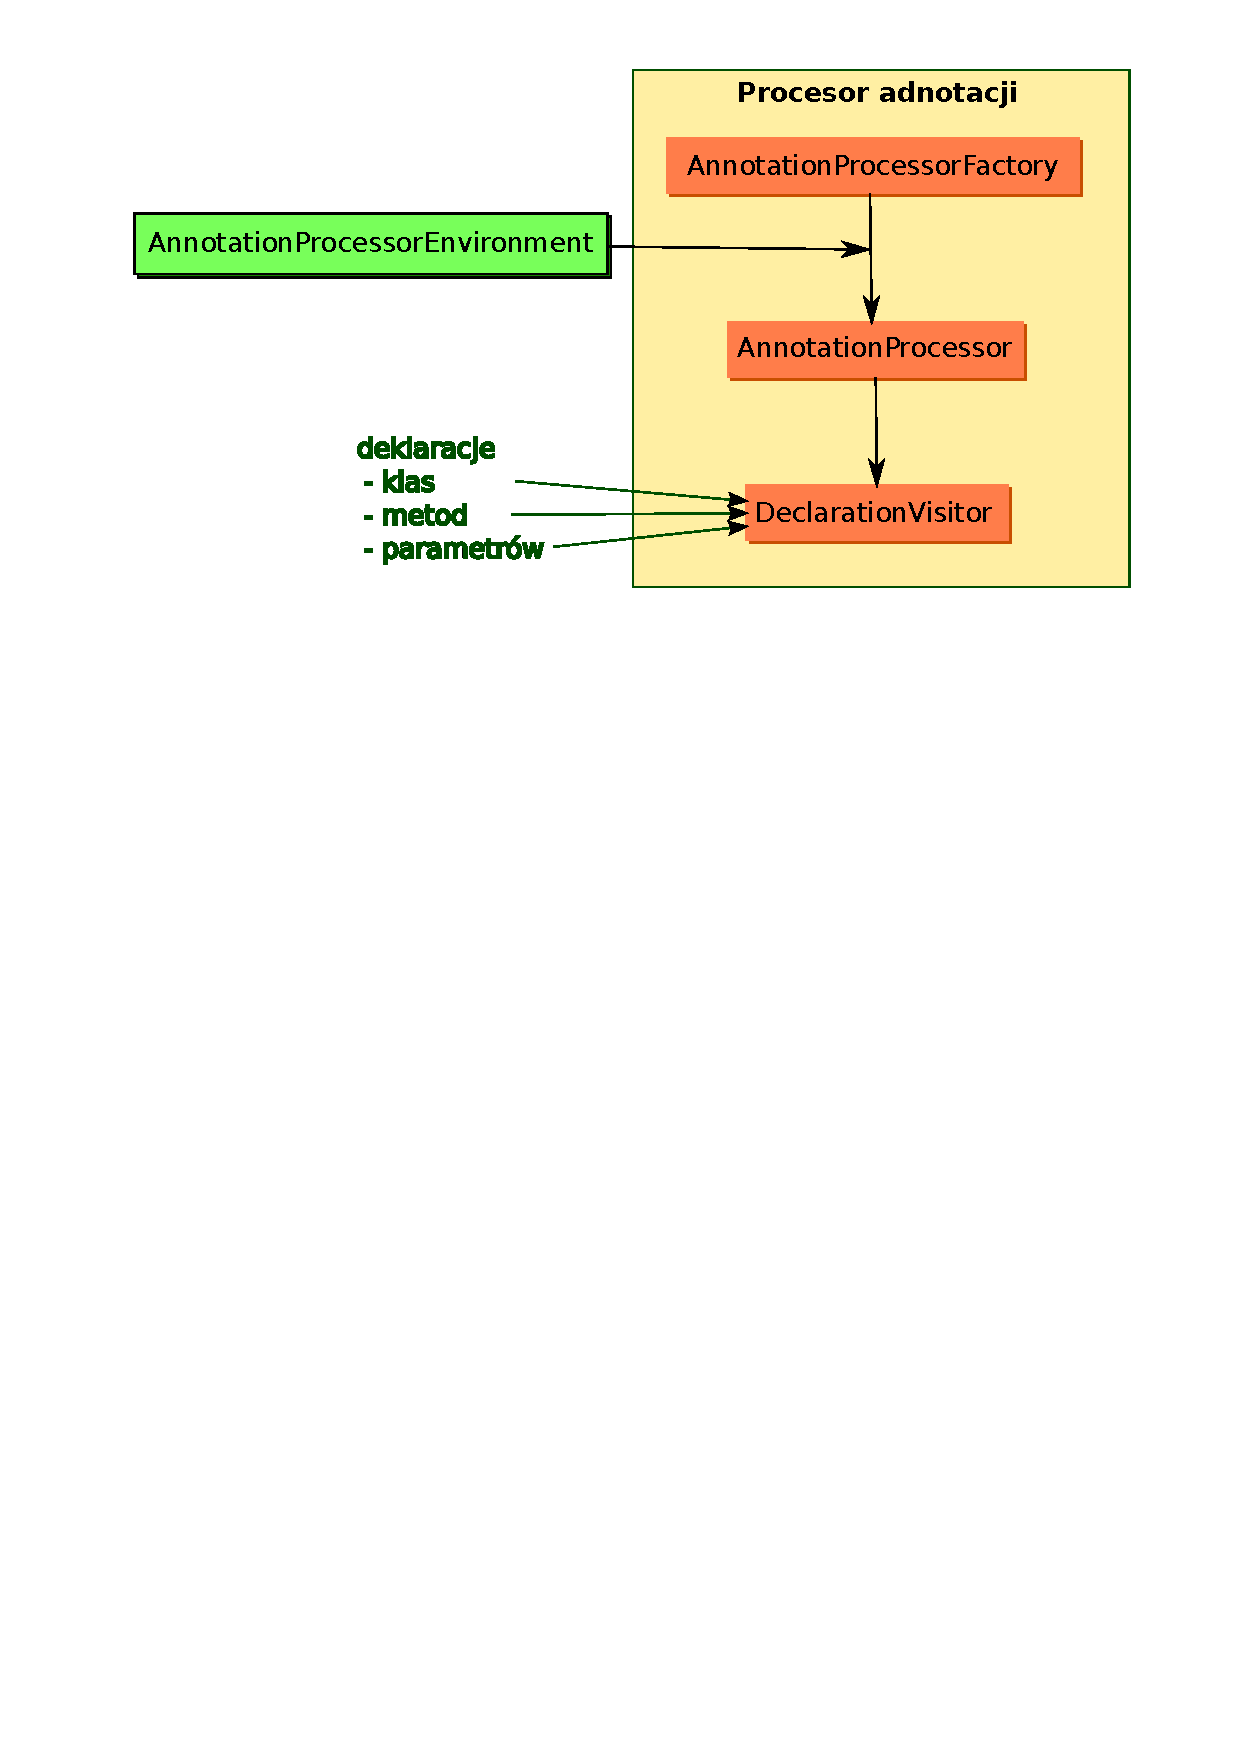
\includegraphics[scale=0.55]{img/apt.pdf}
\end{frame}

\begin{frame}{Ograniczenia}
  \begin{itemize}
  \item Deklaracje przedstawiane procesorowi adnotacji 
    nie pozwalają na dostęp do struktury kodu.
    \begin{itemize}
    \item Brak dostępu do treści metod i konstruktorów
    \end{itemize}
  \item Uniemożliwia to weryfikację adnotacji opisujących zachowanie
    programu. W tym celu należałoby 
    \only<1>{stworzyć}
    \only<2>{\sout{stworzyć}}
    \only<3>{\textbf{znaleźć}} 
    narzędzie, które potrafi przejść całe drzewo składni programu.
  \end{itemize}
\end{frame}
    
\subsection{Checker Framework}

\begin{frame}{Checker Framework}
  \begin{itemize}
  \item Narzędzie do tworzenia i weryfikacji systemów typów 
    opartych o adnotacje zgodne z JSR 308.
  \item Pozwala na definiowanie kwalifikatorów typów i dowodzenie
    własności programów w odniesieniu do obiektów tych typów.
  \end{itemize}
\end{frame}

\begin{frame}{Kwalifikatory typów}
  \textbf{Definicja}
  \lstinputlisting{code/qual-example.java}
  \textbf{Użycie}
  \lstinputlisting{code/qual-usage.java}
\end{frame}
  
\begin{frame}{Hierarchia kwalifikatorów}
  \lstinputlisting{code/qual-hierarchy.java}
  \begin{center}
    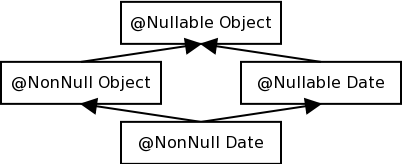
\includegraphics[scale=0.6]{img/nullness.png}
  \end{center}
\end{frame}

\begin{frame}{Sprawdzane własności}
  Checker sprawdza:
  \begin{itemize}
  \item<1-> przypisania:
    \lstinputlisting{code/nonnull-invalid.java}
  \item<2-> wywołania metod
  \item<2-> argumenty typów generycznych
  \item<3-> inne własności zdefiniowane przez checker:
    \lstinputlisting{code/nonnull-invalid-deref.java}
  \end{itemize}
\end{frame}

\begin{frame}{Istniejące checkery}
\begin{itemize}
\item<1-> Nullness
\item<2-> wzajemne wykluczanie -- monitory
\item<3-> niemodyfikowalność obiektów
\item<4-> \emph{taint}
\end{itemize}
\end{frame}

\section{Praca magisterska}

\subsection{Wprowadzenie}

\begin{frame}{Praca magisterska}
\begin{center}
  \textbf{Weryfikacja funkcyjności metod Javy}\\
  w oparciu o system typów z pracy \emph{Functional Java}
\end{center}
\end{frame}

\begin{frame}{Funkcyjność}
  Co to jest metoda \emph{funkcyjna}?
  \begin{itemize}
  \item<1-> nie modyfikuje stanu,
  \item<2-> wywołana z tymi samymi argumentami, zawsze da ten sam wynik.
  \end{itemize}
\end{frame}

\begin{frame}{Motywacja}
  Dlaczego chcemy funkcyjnych metod?
  \begin{itemize}
  \item<1-> ich wywołanie nie może naruszyć niezmienników,
  \item<2-> wywołanie jest bezpieczne w środowisku wielowątkowym, 
  \item<2-> brak wyścigów o dane,
  \item<3-> bezpieczne w niezaufanym środowisku.
  \end{itemize}
\end{frame}

\subsection{JaFun}

\lstset{morekeywords={class,func,immutable,lstate,rep,let,in}}
\begin{frame}{Przykład}
  \lstinputlisting{code/jafun.java}
\end{frame}

\begin{frame}{Weryfikacja kwalifikatorów}
  \structure{Poprawność programu}
  \begin{prooftree}
    \RightLabel{$(prog)$}
    \AxiomC{$\forall_{C\in\overline{C}} \vdash C : ok$}
    \UnaryInfC{$\vdash \overline{C} : ok$}
  \end{prooftree}
  \structure{Poprawność metody}
  \begin{prooftree}
    \AxiomC{$Ex = \text{throws}(\overline{C}, C, M)\quad\quad \forall_{D\in Ex} D\in\overline{C}$}
    \noLine
    \UnaryInfC{$Loc = \text{par2loc}(\text{params}(\overline{C},C,M))$}
    \noLine
    \UnaryInfC{$m=\text{name}(\overline{C},C,M) \quad\quad \text{mmod}=\text{modifier}(\overline{C},C,M)$}
    \noLine
    \UnaryInfC{$\overline{C};C:\text{cmod}, m:\text{mmod}; Ex; Loc
      \vdash \text{body}(\overline{C},C,M) : \text{mok}$}
    \UnaryInfC{$\overline{C}; C : \text{cmod} \vdash M : \text{ok}$}
  \end{prooftree}
\end{frame}

\begin{frame}{Weryfikacja kwalifikatorów}
  \structure{Poprawność wywołania metody w metodzie funkcyjnej}
  \begin{prooftree}
    \AxiomC{$C_1, C_2 \in\overline{C}$}
    \AxiomC{$x : \left<C_1, \tau_1, \tau_2\right>\in Loc$}
    \noLine
    \BinaryInfC{$\text{modifier}(\overline{C},C_1,m')=\textbf{func}$}
    \noLine
    \UnaryInfC{$\overline{C}; C : \text{cmod}, m : \textbf{func}; 
      Ex, Loc\vdash x.m'(\overline{x}) : C_2$}
    \UnaryInfC{$\overline{C}; C :\, \text{cmod}, m : \textbf{func}; 
      Ex; Loc\vdash x.m'(\overline{x}) : \text{mok}$}
  \end{prooftree}
\end{frame}

\subsection{Funcheck}

\begin{frame}{Zadania}
  \begin{itemize}
  \item<1-> Reguły dowodzenia dla Javy
    \pause
    \begin{itemize}
      \item ...albo jej podzbioru.
      \item JaFun nie ma np. składania instrukcji ani przypisań
    \end{itemize}
  \item<3-> Wprowadzanie własności z JaFun do kodu Javy
    \pause
    \begin{itemize}
    \item Adnotacje! \\
      {\color{annot} @Function}, 
      {\color{annot} @Representation}, 
      {\color{annot} @LocalState}
    \end{itemize}
  \item<5-> Checker
  \end{itemize}
\end{frame}

\begin{frame}{Projekt checkera}
  \begin{center}
    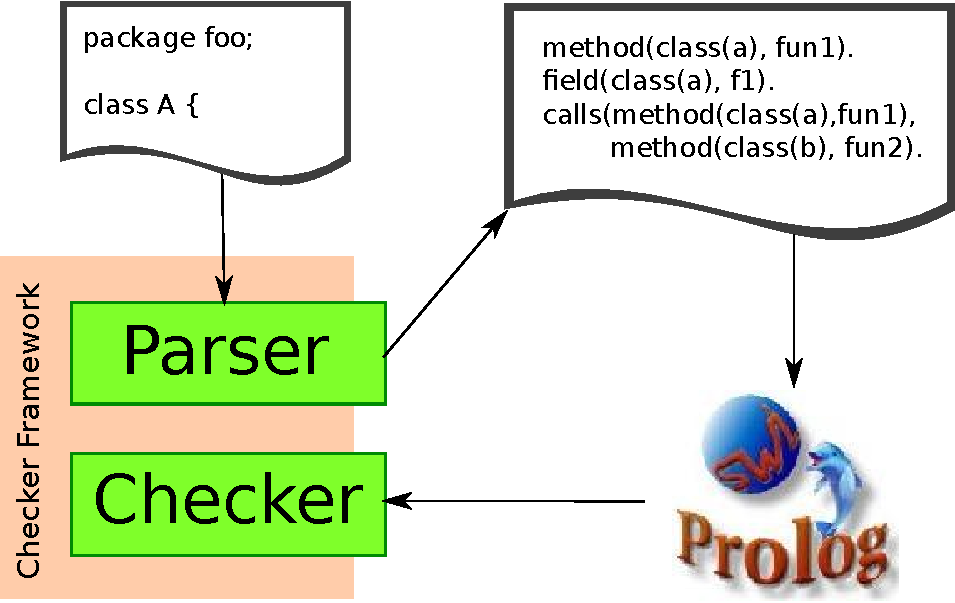
\includegraphics[scale=0.6]{img/project.pdf}
  \end{center}
\end{frame}

\begin{frame}{Dalsze losy}
Rozwój projektu można obserwować w publicznym repozytorium:
\begin{center}
\vspace{3mm}
\structure{www.github.com/saf/Funcheck}\\
\vspace{3mm}
\texttt{git clone git://github.com/saf/Funcheck.git}
\end{center}
\end{frame}

\begin{frame}{Bibliografia}
  \begin{itemize}
  \item M. D. Ernst, \emph{Type Annotations Specification (JSR 308)}, 
  \item \emph{The Checker Framework: Custom pluggable types for Java}
  \item J. Chrząszcz, A. Schubert, \emph{Functional Java}
  \item M. Nygard, \emph{When Should You Jump? JSR 308. That's When.} [w:] ``Wide Awake Developers'', 6 maja 2008.
  \end{itemize}
\end{frame}

\end{document}
